% % ----------------------------------------------------------------------- %
% % Arquivo: 6-implantacao-no-ifsc.tex
% % ----------------------------------------------------------------------- %

% \chapter{Plano de implantação da infraestrutura de serviços proposta}
% \label{implantacao_no_ifsc}

% O capítulo anterior demonstra que a utilização do Rook - mesmo que ainda em estágio de desenvolvimento - pode satisfazer as necessidades de armazenamento persistente de serviços via blocos e objetos, podendo assim ser utilizado na infraestrutura de serviços proposta para o \ac{IFSC}.

% A implementação da infraestrutura de contêineres proposta para o \ac{IFSC} caracteriza-se como um processo contínuo de melhoria, o qual deve ser planejado a longo prazo e ter apoio de diversos setores da instituição, haja vista que é preciso que haja não apenas uma reorganização da infraestrutura da instituição, mas também uma alteração na governança de \ac{TI}.

% Como mostrado na \autoref{fluxograma_implantacao}, o plano de implantação da infraestrutura de serviços proposta para o \ac{IFSC} divide-se em quatro etapas principais: adequação das políticas de \ac{TI} do \ac{IFSC}, implementação de nuvens de contêineres locais nos câmpus da instituição, integração das nuvens locais e utilização da nova infraestrutura no ambiente de produção. Estas etapas são descritas nas subseções a seguir.

% \begin{figure}[!htpb]
% 	\centering
% 	\caption{Fluxograma de implantação da infraestrutura proposta no \ac{IFSC}}
%     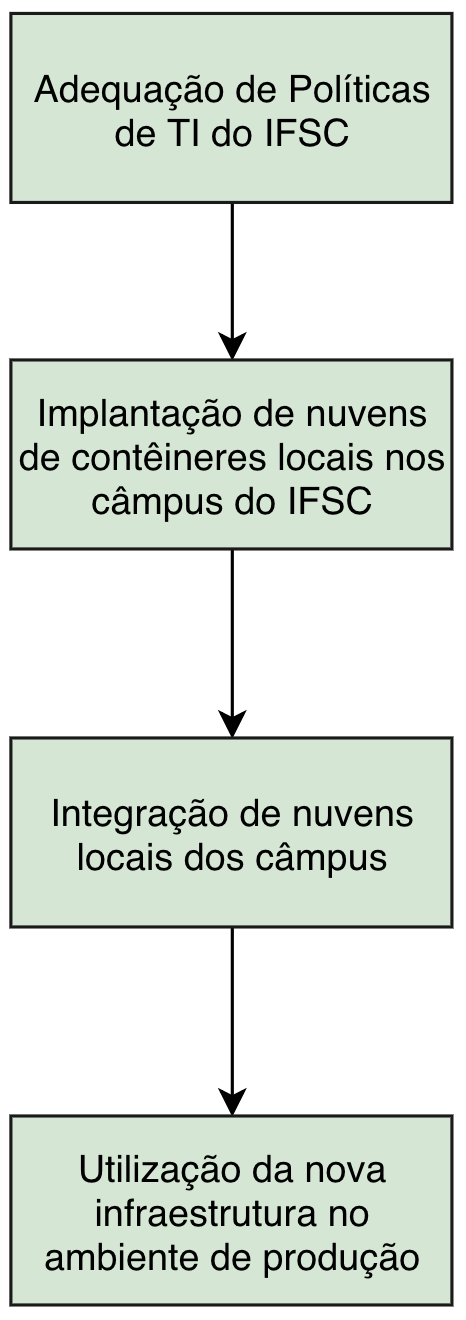
\includegraphics[height=13cm]{TCC/figuras/6-plano/Fluxograma-Plano_IFSC}
    
% 	Fonte: Elaborado pelo autor.
%  	\label{fluxograma_implantacao}
% \end{figure}

% \section{Adequação das Políticas de TI}

% A formação de funcionários para melhoria da infraestrutura dos câmpus e a melhoria das infraestruturas em si caracterizam-se como o primeiro passo do plano de implantação da infraestrutura de serviços baseadas em contêineres proposta para o \ac{IFSC}.

% Devido a descentralização da infraestrutura de serviços proposta para a instituição será necessário que haja uma alta coordenação entre os departamentos de \ac{TIC} para manutenção e expansão do sistema. É importante ressaltar que as funções destes departamentos nos câmpus do \ac{IFSC} permanecerão as mesmas, sendo que as funções dos departamentos na manutenção da infraestrutura - até o momento local e física - também permanecerão os mesmas, mas agora em um ambiente virtual e descentralizado.

% É possível observar na \autoref{organograma_ifsc} que as \ac{CTIC}s estão abaixo dos departamentos de administração dos câmpus onde elas se encontram. Isto significa que a influência da \ac{DTIC} sobre estes departamentos dá-se principalmente através das políticas de governança e do \ac{PDTI} da instituição, visto que a \ac{DTIC} não é diretamente responsável pelas \ac{CTIC}s de cada câmpus.

% \begin{figure}[!htpb]
% 	\centering
% 	\caption{Organograma simplificado dos departamentos de \ac{TIC} do \ac{IFSC}}
%     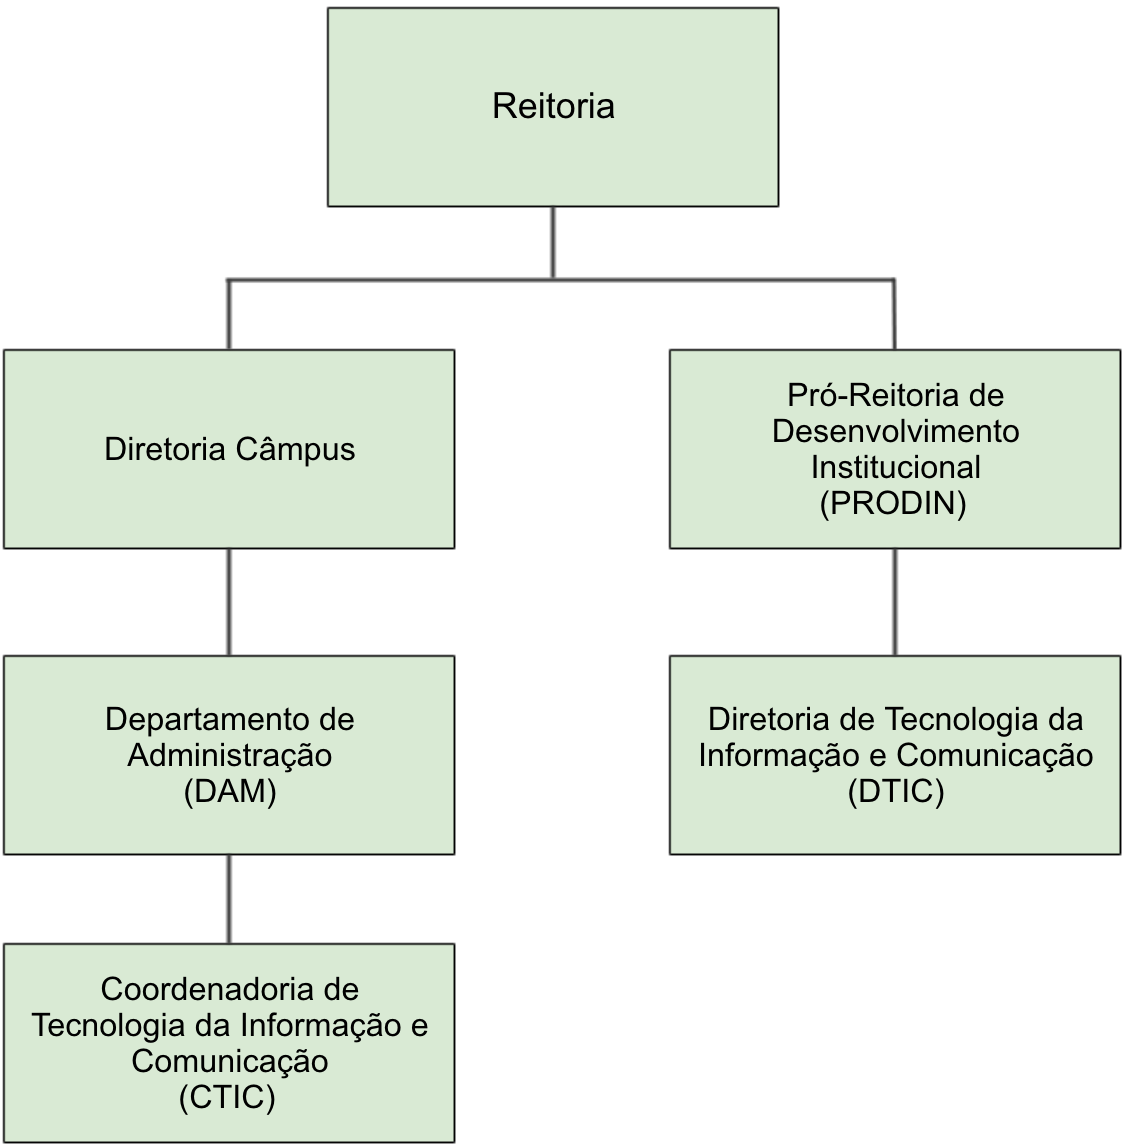
\includegraphics[width=11cm]{TCC/figuras/6-plano/Organograma-CTIC_DTIC}
    
% 	Fonte: Elaborado pelo autor.
%  	\label{organograma_ifsc}
% \end{figure}

% Propõe-se, portanto, que sejam adicionadas ao \ac{PDTI} ações que promovam a formação dos funcionários focada nas necessidades de infraestrutura dos câmpus, resultado assim no alinhamento dos serviços e infraestruturas da instituição. Na prática a convergência das infraestruturas locais facilitará a sua posterior integração e manutenção, o que é vantajoso para a instituição. 

% É importante ressaltar que o \ac{PDTI} já promove ações para formação de funcionários da instituição. De acordo com o \ac{PDTI} de 2018, por exemplo, o plano a executar em 2018 para capacitação promove diversos cursos para formação dos funcionários, tais como ``IOS SWIFT BOOTCAMP'' e ``Mobile Apps para iOS e Android com HTML5 e PhoneGap'' \cite{pdti2018}. Sugere-se que cursos nas áreas de ``Segurança de Redes e Sistemas'' e ``Administração e Projetos de Redes'' (também ofertados atualmente) tenham mais enfoque, visando melhorar as infraestruturas locais dos câmpus para melhor integração futura dos serviços. Pode-se, por exemplo, classificar as necessidades de cada câmpus da instituição e atribuir-se prioridades a cada necessidade, facilitando assim a escolha de cursos de formação e treinamento para funcionários do \ac{IFSC} baseados nestas prioridades. Caso possível, os cursos de formação nas áreas propostas podem ser ofertados por funcionários da própria instituição, economizando assim recursos que seriam gastos em cursos externos.

% \section{Implantação de nuvens de contêineres locais nos câmpus}

% O segundo passo na implantação da infraestrutura proposta é que sejam implantadas nuvens de contêineres locais em cada câmpus da instituição. Estas nuvens serão nuvens de testes, as quais possibilitarão que funcionários da instituição se familiarizem com nuvens de contêineres, além de possibilitar testes de portabilidade dos serviços atualmente ofertados pela instituição para este ambiente.

% Alguns dos serviços ofertados pela instituição podem ser facilmente implementados em nuvens de contêineres através da utilização de versões (imagens) estáveis das aplicações, como o Moodle e a plataforma de e-mail Zimbra, por exemplo. Outros serviços, como o \ac{SIG}, precisarão ser portados para a forma de contêiner. Esta etapa do planejamento caracteriza-se, portanto, como o estudo das tecnologias que serão utilizadas na infraestrutura e adequação destas tecnologias ao cenário do \ac{IFSC}.

% É importante ressaltar que a comunidade acadêmica também pode ser envolvida nesta etapa, incentivando tanto professores quanto alunos a conduzir projetos e trabalhos de conclusão de curso que colaborem com o projeto (a exemplo deste trabalho).

% \section{Integração de nuvens de contêineres locais dos câmpus}

% A terceira etapa da implantação da infraestrutura de serviços proposta é a integração das nuvens locais de cada câmpus. Isto permitirá que tenha-se um melhor entendimento das necessidades do sistema, tanto do posto de vista de administração do sistema quanto de recursos físicos necessários para a realização do projeto.

% Nesta etapa poderão ser discutidas e determinadas as funções de cada câmpus/funcionário na manutenção do sistema, delegando funções específicas para membros das equipes de \ac{TIC} que participarem diretamente na administração do sistema. Por exemplo, um membro do departamento da \ac{CTIC} do câmpus São José poderá ser responsável pela administração do serviço Moodle, enquanto outro membro da \ac{CTIC} do câmpus Florianópolis será responsável pela administração da rede da nuvem (a qual poderá ser uma rede virtual através da utilização de \ac{SDN}).

% Também será possível determinar as necessidades de \textit{hardware} de cada câmpus, podendo realizar a aquisição de novos equipamentos ou redistribuição de equipamentos entre os câmpus da instituição. Caso seja determinado que é necessário adquirir novos equipamentos deve-se optar pela aquisição de \textit{hardware} com \textit{design} modular, ou seja, equipamentos que permitam fácil reposição e aprimoramento de módulos utilizados. No cenário de armazenamento, por exemplo, deverão ser utilizados equipamentos que permitam o aprimoramento do armazenamento tanto em relação a capacidade de armazenamento quanto a tecnologia de armazenamento utilizada (como \ac{SSD}, por exemplo).

% A integração de infraestruturas também permitirá que seja realizada uma análise ampla do sistema em relação aos \textit{softwares} e serviços utilizados no \ac{IFSC}. \textit{Softwares} proprietários que requerem a compra de licenças, como o MATLAB, por exemplo, poderão ser implantados na infraestrutura de contêineres, possibilitando assim que a instituição não precise de licenças individuais a serem utilizadas em cada câmpus, mas sim de licenças que possam ser utilizadas de forma coletiva através da infraestrutura de serviços proposta.

% \section{Utilização da nova infraestrutura no ambiente de produção}

% Após a integração de infraestruturas e estabilização do sistema será possível iniciar a utilização do novo ambiente na produção. 

% A utilização da nova infraestrutura deverá ocorrer de forma gradual. Primeiramente será necessário migrar os dados armazenados da infraestrutura atual para a nova infraestrutura. Após esta migração será possível realizar o balanceamento de carga dos serviços entre a infraestrutura atual e a de contêineres, sendo que a infraestrutura de contêineres deverá a princípio receber pouco tráfego e requisições para que seja possível avaliar seu desempenho e otimizar o sistema conforme necessário. Este balanceamento de carga também ocorrerá de forma gradual, sendo que a utilização da infraestrutura de contêineres irá crescer de acordo com sua otimização e estabilização. Após comprovar-se que a nova infraestrutura é estável e atende às necessidades da instituição de forma satisfatória e eficaz será possível desativar a infraestrutura atual, completando assim o ciclo de implantação da infraestrutura de contêineres no \ac{IFSC}.